\chapter{Phương pháp đề xuất}
\label{chap:methodology}

\section{Tổng quan hướng tiếp cận}\label{sec:tongquan}

Đầu vào của mọi mô hình ước lượng là 16 đặc trưng đoạn sạc và chỉ số chu kỳ (\Cref{ch:dactrung}). Mọi mô hình được đánh
giá trong cùng một giao thức không rò rỉ: kiểm định chéo theo cell, lặp lại nhiều lần, so ghép cặp theo cell
(\Cref{sec:protocol}). Mô hình đề xuất cho bài toán ước lượng là PINN bán giám sát (\Cref{sec:pinn}), trong đó hàm mất
mát vật lý của một động học suy giảm dạng xám được tính trên cả cell không có nhãn. Mô hình kết hợp PINN-lai ghép ba
PINN-semi với GBDT rồi lọc xu thế (\Cref{sec:pinnlai}). Các mô hình đối chứng gồm Ridge, GPR, GBDT, MLP, CNN, LSTM,
Transformer và các biến thể PINN (\Cref{sec:baselines}). Mốc so sánh với công trình gốc là PINN4SOH trên đúng cách chia
của bài (\Cref{ch:sosanh}). Phần mở rộng xét ba câu hỏi gần với vận hành BMS: đo dung lượng thưa trên mọi cell thay vì
đo đầy đủ một phần cell, cập nhật ước lượng khi cell mới được đo vài lần, và dự báo SOH, dung lượng, RUL
(\Cref{sec:mo_rong,sec:e33pp}).

\section{Dữ liệu và đặc trưng đầu vào}\label{ch:dactrung}

Mục này mô tả bốn bộ dữ liệu và cách tiền xử lý, liệt kê các đặc trưng được dùng, rồi trình bày các phương pháp và số
liệu cho thấy vì sao dùng chúng và vì sao bỏ các đặc trưng hay cách biến đổi khác.

\subsection{Bốn bộ dữ liệu}\label{sec:data}

Cả bốn bộ là cell hình trụ 18650 được sạc--xả lặp lại trong phòng thí nghiệm tới khi dung lượng giảm sâu.
\begin{itemize}
\item XJTU, Đại học Giao thông Tây An, công bố cùng PINN4SOH~\cite{wang2024}: 55 cell NCM, danh định 2,0\,Ah, sáu chế độ
      thí nghiệm (sạc 2C, sạc 3C, xả ngẫu nhiên R2.5 và R3, bước ngẫu nhiên RW, mô phỏng quỹ đạo vệ tinh) ở nhiệt độ phòng.
\item TJU, Zhu và cộng sự~\cite{zhu2022}: 130 cell thuộc ba nhóm hoá học (NCA, NCM, NCM+NCA), thử ở 25, 35 và
      45\,\textdegree C với nhiều tốc độ sạc, tạo thành chín nhóm điều kiện.
\item MIT, Severson và cộng sự~\cite{severson2019}: cell LFP/graphite 1,1\,Ah, nhiều giao thức sạc nhanh, ba đợt thí
      nghiệm, buồng nhiệt 30\,\textdegree C.
\item HUST, Ma và cộng sự~\cite{ma2022}: 77 cell LFP/graphite 1,1\,Ah, cùng chế độ sạc nhanh và 77 chế độ xả nhiều bước
      khác nhau, 30\,\textdegree C.
\end{itemize}
Đặc trưng đoạn sạc của cả bốn bộ được trích theo cùng một quy trình và công bố kèm PINN4SOH, nên bốn bộ có chung không
gian đặc trưng. Bảng~\ref{tab:datastats} tóm tắt dữ liệu sau tiền xử lý.

\begin{table}[!htbp]\centering\footnotesize
\caption[Thống kê bốn bộ dữ liệu sau tiền xử lý]{Thống kê bốn bộ dữ liệu sau tiền xử lý. “Nhóm” là số chế độ thí nghiệm khác nhau dùng để phân tầng.}\label{tab:datastats}
\begin{adjustbox}{max width=\textwidth}\begin{tabular}{llrrrcccc}\toprule
Bộ & Hoá học & Cell & Chu kỳ & Nhóm & Tuổi thọ (min / trung vị / max) & SOH đầu & SOH cuối & $Q_\text{dđ}$ (Ah) \\\midrule
XJTU & NCM & 55 & 22.431 & 6 & 110 / 392 / 942 & 0{,}83--1{,}00 & 0{,}78--0{,}89 & 2,0 \\
TJU & NCA/NCM & 130 & 56.697 & 9 & 25 / 377 / 1.246 & 0{,}88--0{,}98 & 0{,}66--0{,}90 & 3,5 / 2,5 \\
MIT & LFP & 125 & 82.450 & 3 & 36 / 622 / 2.156 & 0{,}95--1{,}00 & 0{,}82--0{,}97 & 1,1 \\
HUST & LFP & 77 & 144.224 & 1 & 1.123 / 1.855 / 2.672 & 1{,}06--1{,}12 & 0{,}80--0{,}82 & 1,1 \\
\textbf{Tổng} &  & 387 & 305.802 &  &  &  &  &  \\
\bottomrule\end{tabular}\end{adjustbox}\end{table}


\subsection{Tiền xử lý}\label{sec:prep}

Nhãn của chu kỳ $n$ trong cell $c$ là $y_{c,n} = Q_{c,n}/Q_\text{danh định}$. Chu kỳ thiếu dung lượng được giữ lại với
nhãn trống và chỉ dùng cho hàm mất mát vật lý.

Dữ liệu sạc có thể có những chu kỳ bất thường, ví dụ do lỗi đo hoặc lỗi ghi làm một đặc trưng nhảy vọt rồi trở lại. Các
chu kỳ này được bỏ trước khi học bằng một bộ lọc ngoại lai nhân quả. Chu kỳ $n$ bị loại nếu có đặc trưng không hữu hạn,
hoặc có đặc trưng lệch xa so với 50 chu kỳ liền trước của chính cell. Với đặc trưng thứ $j$:
\begin{equation}
m_{n,j} = \operatorname{median}(x_{n-50..n-1,\,j}), \quad
s_{n,j} = \max\!\Big(\tfrac{\mathrm{IQR}(x_{n-50..n-1,\,j})}{1{,}349},\, 0{,}01\,|m_{n,j}|\Big), \quad
z_{n,j} = \frac{|x_{n,j} - m_{n,j}|}{s_{n,j}},
\end{equation}
và chu kỳ bị loại nếu $\max_j z_{n,j} > 5$. Ở đây $s_{n,j}$ là độ lệch chuẩn ước lượng bền vững: với phân phối chuẩn,
IQR$/1{,}349$ bằng đúng độ lệch chuẩn, nhưng không bị chính các chu kỳ bất thường kéo lên như độ lệch chuẩn thường. Sàn
$1\,\%\,|m_{n,j}|$ tránh chia cho số gần 0 ở đặc trưng gần như không đổi. Bộ lọc chỉ chạy khi đã có ít nhất 10 chu kỳ
lịch sử, vì trung vị và IQR của ít điểm hơn dao động mạnh. Vì vậy 10 chu kỳ đầu của mỗi cell không bị lọc. Ngưỡng là 5
thay cho 3 quen dùng, vì độ lệch chuẩn ở đây chỉ tính trên 50 chu kỳ gần nhất, nhỏ hơn nhiều độ lệch chuẩn của cả vòng
đời vốn bị xu thế suy giảm làm lớn lên. Ngưỡng được ấn định trước khi huấn luyện, để tỉ lệ chu kỳ bị loại (1{,}6\,\%)
tương đương bộ lọc $3\sigma$ dùng cả vòng đời (2{,}2\,\%). Bộ lọc chỉ nhìn đặc trưng, không nhìn dung lượng, và chỉ nhìn
quá khứ của cell, nên chạy được khi đang dùng và không rò rỉ. Ở cách đặt này, tỉ lệ chu kỳ bị loại là 3{,}1\,\% (XJTU), 1{,}3\,\% (TJU), 3{,}7\,\% (MIT), 0{,}1\,\% (HUST). Một kiểm tra sau, không dùng để chọn tham số (GBDT, 30\,\% nhãn, 3 lần lặp $\times$ 5 fold, MAE chấm trên cùng một tập chu kỳ test cho mọi cách đặt, Wilcoxon ghép cặp theo cell, Holm qua bốn bộ): đổi ngưỡng thành 3, 4, 6 hoặc 8 làm tỉ lệ chu kỳ bị loại đi từ 5{,}7--18{,}5\,\% (ngưỡng 3) tới 0{,}0--1{,}1\,\% (ngưỡng 8), còn MAE bằng 0{,}993--1{,}035 lần cách đặt của đồ án, cao hơn có ý nghĩa ở 4 trên 16 trường hợp, không trường hợp nào thấp hơn có ý nghĩa; bỏ hẳn bước lọc cho MAE bằng 0{,}998--1{,}045 lần (cao hơn có ý nghĩa ở 1 trên 4 bộ); đổi số chu kỳ lịch sử tối thiểu thành 5 hoặc 20 cho 0{,}993--1{,}021 lần (cao hơn có ý nghĩa ở 2 trên 8 trường hợp, thấp hơn có ý nghĩa ở 1).


Mỗi đặc trưng được chuẩn hoá z-score bằng trung bình và độ lệch chuẩn tính trên các cell huấn luyện của fold, gồm cả cell
có nhãn và không nhãn: $\tilde{\mathbf{x}} = (\mathbf{x} - \boldsymbol\mu)/(\boldsymbol\sigma + 10^{-6})$. Biến thời gian
là $t_n = n/1000$ với $n$ là chỉ số chu kỳ gốc. Hằng số 1000 dùng chung cho mọi cell.

\subsection{Các đặc trưng được dùng}\label{sec:dt_dung}

Mọi mô hình ước lượng SOH của đồ án nhận cùng 17 đầu vào: 16 đặc trưng đoạn sạc ở Bảng~\ref{tab:features} và biến thời
gian $t$. Mô hình chuỗi nhận thêm các chu kỳ trước của chính cell. Nhiệt độ không phải đầu vào của mạng nghiệm. Ở
PINN-semi, nhiệt độ chỉ xuất hiện trong thừa số Arrhenius của động học suy giảm (Mục~\ref{sec:pinn}).

\begin{table}[!htbp]\centering\small
\caption[Các đặc trưng đầu vào]{Các đặc trưng đầu vào, chia thành bốn nhóm dùng cho phép thử bỏ nhóm ở
Mục~\ref{sec:dt_bonhom}.}\label{tab:features}
\begin{tabularx}{\textwidth}{>{\raggedright}p{3.0cm}>{\raggedright}p{5.4cm}>{\raggedright\arraybackslash}X}
\toprule
Nhóm & Đặc trưng & Ý nghĩa \\
\midrule
V: điện áp pha CC (6) & trung bình, độ lệch chuẩn, độ nhọn, độ bất đối xứng, độ dốc, entropy & hình dạng đường điện áp trong
cửa sổ điện áp của pha dòng không đổi \\
I: dòng điện pha CV (6) & trung bình, độ lệch chuẩn, độ nhọn, độ bất đối xứng, độ dốc, entropy & hình dạng đường dòng điện trong
cửa sổ dòng của pha áp không đổi \\
QT: điện lượng và thời gian (4) & điện lượng nạp và thời gian của pha CC; của pha CV & cell nhận được bao nhiêu điện
lượng và trong bao lâu ở mỗi pha \\
t: thời gian (1) & $t = n/1000$ & tuổi của cell tính bằng số chu kỳ \\
\bottomrule
\end{tabularx}
\end{table}

Có ba lý do chọn bộ đầu vào này trước khi xét số liệu. Thứ nhất, cả 17 đầu vào tính được ở mọi chu kỳ từ dữ liệu BMS ghi
lúc sạc và từ bộ đếm chu kỳ, không cần đo dung lượng. Thứ hai, bốn bộ có chung 16 đặc trưng, nên cùng một mô hình chạy
được trên cả bốn. Thứ ba, đây đúng là đầu vào của PINN4SOH, nên so sánh với bài gốc chỉ khác ở mô hình và cách đánh giá.
Bản dữ liệu đồ án dùng là bản đã trích đặc trưng công bố kèm PINN4SOH, chỉ chứa 16 đặc trưng này và dung lượng. Các đặc
trưng cần đường cong đầy đủ, như đường cong dung lượng gia tăng $\mathrm{d}Q/\mathrm{d}V$ hay điện áp hồi phục sau sạc, đòi
hỏi tải và xử lý lại dữ liệu thô của từng bộ, việc mà đồ án chưa làm. Các mục sau kiểm tra bằng số liệu rằng mỗi nhóm
đều mang thông tin, và rằng các đặc trưng hay cách biến đổi khác đã thử đều không nên dùng.

\subsection{Phương pháp kiểm tra}\label{sec:dt_pp}

Đồ án dùng bốn phép kiểm tra trên cùng dữ liệu đã tiền xử lý ở Mục~\ref{sec:prep}.
\begin{enumerate}
\item Mức liên quan và trùng lặp, một phương pháp lọc không cần mô hình. Với mỗi đặc trưng, hệ số Spearman $\rho$ giữa
      đặc trưng và SOH được tính theo hai cách: trong từng cell rồi lấy trung vị qua các cell (kèm tỉ lệ cell có
      $|\rho| \ge 0{,}5$), và trên mọi chu kỳ của bộ. Hai đặc trưng có $|\rho| \ge 0{,}95$ với nhau trên mọi chu kỳ của
      bộ được coi là gần như trùng thông tin.
\item Bỏ hoặc thêm nhóm, một phương pháp bao. GBDT được huấn luyện lại với từng tập đầu vào trên đúng các fold không rò rỉ
      của đồ án (5 fold theo cell, lần lặp 0--2, cùng tập cell có nhãn), ở hai mức nhãn 10 và 70\,\% số cell. MAE theo
      cell trên tập kiểm tra được so với bộ đầy đủ bằng kiểm định Wilcoxon ghép cặp theo cell, hiệu chỉnh Holm qua bốn
      bộ. GBDT được chọn vì là mô hình đơn lẻ mạnh nhất của đồ án (Mục~\ref{sec:labels}) và đủ nhanh để huấn luyện lại
      hàng trăm lần. Với đủ 17 đầu vào, dự đoán của nó giống hệt GBDT trong các thí nghiệm chính, nên hàng đầu của
      Bảng~\ref{tab:ablation} trùng cột GBDT của Bảng~\ref{tab:allmae}, cùng 3 lần lặp. Bảng~\ref{tab:big} lấy trung bình
      5 lần lặp nên có số khác đôi chút.
\item Độ quan trọng hoán vị trên tập kiểm tra của mô hình đầy đủ: hoán vị một đặc trưng, hoặc cả một nhóm, giữa các hàng
      kiểm tra và đo tỉ số MAE theo cell sau và trước hoán vị.
\item Chọn đặc trưng trên tập xác thực: trong mỗi fold, bỏ các đặc trưng mà hoán vị trên tập xác thực làm sai số tăng
      dưới 1\,\%, huấn luyện lại và đánh giá trên tập kiểm tra. Đây là cách chọn đặc trưng tự động không chạm tới tập
      kiểm tra.
\end{enumerate}
Các cách biến đổi đầu vào khác (chuẩn hoá theo cả vòng đời cell, đặc trưng tương đối, đặc trưng có lịch sử) được kiểm tra
bằng các thí nghiệm riêng nêu ở Mục~\ref{sec:dt_bo}.

\subsection{Mức liên quan và trùng lặp}\label{sec:dt_lienquan}

Bảng~\ref{tab:relevance} cho thấy trong từng cell, chỉ số chu kỳ gần như tỉ lệ nghịch với SOH ($\rho$ trung vị từ −1{,}00 đến −0{,}94), điều dễ hiểu vì SOH giảm dần theo thời gian. Nhiều đặc trưng sạc cũng biến thiên chặt theo SOH; số đặc trưng có $|\rho|$ trung vị từ 0,9 trở lên là 4 ở XJTU, 9 ở TJU, 5 ở MIT và 7 ở HUST. Nhưng đặc trưng mạnh nhất không giống nhau giữa các bộ: điện lượng pha CV ở XJTU, thời gian pha CV ở TJU, trung bình điện áp ở MIT và thời gian pha CC ở HUST. Có đặc trưng còn đổi chiều theo hệ hoá học: độ nhọn dòng điện tăng theo SOH ở hai bộ LFP ($\rho$ 0{,}77 và 0{,}87) nhưng giảm ở XJTU và TJU (−0{,}70 và −0{,}98). Không đặc trưng nào yếu ($|\rho| < 0{,}3$) ở cả bốn bộ, nên không có lý do bỏ một đặc trưng chỉ vì tương quan thấp.

Một số cặp đặc trưng gần như trùng nhau ($|\rho| \ge 0{,}95$ trên mọi chu kỳ của bộ): 13 cặp ở XJTU, 4 cặp ở TJU, 3 cặp ở MIT và 14 cặp ở HUST, nhưng chỉ có cặp độ nhọn dòng điện và độ bất đối xứng dòng điện trùng ở cả bốn bộ. Một cặp trùng ở bộ này lại mang hai thông tin khác nhau ở bộ khác, nên với một tập đầu vào chung không thể bỏ cột nào chỉ vì trùng lặp. Trùng lặp cũng làm phép hoán vị từng cột đánh giá thấp tầm quan trọng của mỗi cột trong cặp, vì vậy các phép thử dưới đây bỏ và hoán vị theo nhóm. Ngoài ra, tương quan đơn biến không cho biết một đặc trưng có giúp phân biệt các cell khi đi cùng các đặc trưng khác hay không, nên việc giữ hay bỏ phải được thử trực tiếp bằng mô hình.

\begin{table}[!htbp]\centering\small\setlength{\tabcolsep}{4pt}
\caption[Tương quan hạng giữa từng đầu vào và SOH]{Hệ số Spearman $\rho$ giữa từng đầu vào và SOH: trung vị qua các cell của $\rho$ tính trong từng cell (cột “trong cell”), và $\rho$ trên mọi chu kỳ của bộ (cột “gộp”). Dấu âm: đầu vào giảm khi SOH tăng.}\label{tab:relevance}
\begin{adjustbox}{max width=\textwidth}\begin{tabular}{lrrrrrrrr}\toprule
 & \multicolumn{2}{c}{XJTU} & \multicolumn{2}{c}{TJU} & \multicolumn{2}{c}{MIT} & \multicolumn{2}{c}{HUST} \\\cmidrule(lr){2-3}\cmidrule(lr){4-5}\cmidrule(lr){6-7}\cmidrule(lr){8-9}
Đầu vào & trong cell & gộp & trong cell & gộp & trong cell & gộp & trong cell & gộp \\\midrule
trung bình điện áp & 0{,}56 & 0{,}32 & 0{,}05 & 0{,}19 & −0{,}99 & −0{,}75 & −0{,}94 & −0{,}58 \\
độ lệch chuẩn điện áp & −0{,}51 & −0{,}54 & 0{,}24 & 0{,}27 & −0{,}25 & 0{,}11 & −0{,}91 & −0{,}58 \\
độ nhọn điện áp & 0{,}42 & 0{,}45 & −0{,}56 & −0{,}30 & 0{,}97 & 0{,}55 & 0{,}95 & 0{,}63 \\
độ bất đối xứng điện áp & −0{,}59 & −0{,}32 & 0{,}07 & 0{,}01 & 0{,}97 & 0{,}45 & 0{,}95 & 0{,}63 \\
độ dốc điện áp & −0{,}19 & −0{,}06 & −0{,}95 & −0{,}61 & 0{,}88 & 0{,}28 & 0{,}45 & 0{,}13 \\
entropy điện áp & −0{,}18 & −0{,}05 & 0{,}61 & 0{,}29 & 0{,}78 & 0{,}81 & 0{,}97 & 0{,}78 \\
\addlinespace[2pt]
trung bình dòng điện & 0{,}61 & 0{,}42 & 0{,}88 & 0{,}57 & −0{,}78 & −0{,}52 & −0{,}72 & −0{,}48 \\
độ lệch chuẩn dòng điện & 0{,}64 & 0{,}48 & 0{,}54 & 0{,}41 & −0{,}62 & −0{,}41 & −0{,}39 & −0{,}37 \\
độ nhọn dòng điện & −0{,}70 & −0{,}45 & −0{,}98 & −0{,}59 & 0{,}77 & 0{,}51 & 0{,}87 & 0{,}55 \\
độ bất đối xứng dòng điện & −0{,}63 & −0{,}43 & −0{,}98 & −0{,}59 & 0{,}78 & 0{,}52 & 0{,}87 & 0{,}53 \\
độ dốc dòng điện & −0{,}93 & −0{,}81 & −1{,}00 & −0{,}53 & −0{,}59 & −0{,}10 & 0{,}25 & 0{,}09 \\
entropy dòng điện & −0{,}93 & −0{,}82 & −1{,}00 & −0{,}55 & 0{,}37 & 0{,}35 & 0{,}60 & 0{,}26 \\
\addlinespace[2pt]
điện lượng pha CC & −0{,}10 & −0{,}11 & 0{,}95 & 0{,}57 & 0{,}98 & 0{,}89 & 0{,}97 & 0{,}84 \\
thời gian pha CC & −0{,}09 & −0{,}01 & 0{,}95 & 0{,}74 & 0{,}98 & 0{,}90 & 0{,}97 & 0{,}84 \\
điện lượng pha CV & −0{,}94 & −0{,}82 & −1{,}00 & −0{,}69 & 0{,}34 & 0{,}30 & 0{,}55 & 0{,}24 \\
thời gian pha CV & −0{,}94 & −0{,}82 & −1{,}00 & −0{,}65 & 0{,}59 & 0{,}41 & 0{,}64 & 0{,}30 \\
\addlinespace[2pt]
$t$ (chỉ số chu kỳ) & −0{,}94 & −0{,}74 & −1{,}00 & −0{,}93 & −1{,}00 & −0{,}72 & −1{,}00 & −0{,}92 \\
\bottomrule\end{tabular}\end{adjustbox}\end{table}


\subsection{Bỏ hoặc thêm nhóm đặc trưng}\label{sec:dt_bonhom}

Bảng~\ref{tab:ablation} và Hình~\ref{fig:features} cho kết quả bỏ hoặc thêm nhóm ở 8 trường hợp (4 bộ $\times$ 2 mức nhãn), Bảng~\ref{tab:perm} cho độ quan trọng hoán vị của mô hình đủ 17 đầu vào.

\paragraph{Biến thời gian $t$.} Bỏ $t$ làm sai số tăng có ý nghĩa ở 6 trên 8 trường hợp, nhiều nhất 1{,}35 lần; trường hợp duy nhất có lợi là MIT 10\,\% (tỉ số 0{,}90). Ngược lại, chỉ dùng $t$ mà bỏ hết đặc trưng sạc cho sai số gấp 1{,}20--12{,}33 lần: tuổi của cell một mình không đủ để biết SOH, vì các cell già đi với tốc độ rất khác nhau (tuổi thọ trong mỗi bộ chênh nhau nhiều lần, Bảng~\ref{tab:datastats}). Hoán vị $t$ giữa các hàng test làm sai số tăng 1{,}47--8{,}10 lần, nên mô hình thật sự dùng biến này.

\paragraph{Ba nhóm đặc trưng sạc.} Không có trường hợp nào bỏ một nhóm mà sai số giảm có ý nghĩa. Nhóm V (điện áp pha CC) và nhóm QT (điện lượng, thời gian) mang nhiều thông tin nhất: bỏ nhóm V làm sai số tăng có ý nghĩa ở 6 trên 8 trường hợp, bỏ nhóm QT ở 4 trên 8, có trường hợp gần gấp đôi (1{,}99). Bỏ nhóm I (dòng điện pha CV) chỉ làm sai số tăng có ý nghĩa ở 2 trường hợp. Chỉ giữ nhóm QT và $t$, tức 5 đầu vào, kém bộ đầy đủ có ý nghĩa ở 6 trên 8 trường hợp. Phép hoán vị cho cùng nhận xét: hoán vị nhóm QT làm sai số tăng tới 18{,}82 lần, nhóm V tới 5{,}02 lần, nhóm I chỉ tới 3{,}00 lần.

\paragraph{Chọn đặc trưng tự động.} Khi bỏ các đầu vào mà hoán vị trên validation làm sai số tăng dưới 1\,\%, mỗi fold giữ lại trung vị 7--17 trên 17 đầu vào tuỳ bộ và mức nhãn; hay bị bỏ nhất là trung bình dòng điện, độ lệch chuẩn dòng điện và độ lệch chuẩn điện áp. Trên test, cách chọn này cho sai số bằng 0{,}99--1{,}02 lần bộ đầy đủ, không khác có ý nghĩa ở trường hợp nào, tức bớt đầu vào không làm mô hình tốt lên.

\paragraph{Đọc kết quả.} Mọi tập rút gọn đều kém bộ đầy đủ ở ít nhất một trường hợp, và các trường hợp có lợi (bỏ $t$ ở MIT 10\,\%; thêm 16 đặc trưng tương đối ở TJU 70\,\%) không lặp lại ở bộ khác. Chọn đầu vào riêng cho từng bộ dựa trên những kết quả này là chọn mô hình trên tập test, còn chọn riêng cho từng fold bằng validation thì không cải thiện. Vì vậy đồ án dùng chung bộ 17 đầu vào cho mọi bộ dữ liệu và mọi mô hình.

\begin{table}[!htbp]\centering\small\setlength{\tabcolsep}{4pt}
\caption[Bỏ hoặc thêm nhóm đầu vào với GBDT]{Bỏ hoặc thêm nhóm đầu vào, GBDT trên đúng các fold không rò rỉ (3 lần lặp $\times$ 5 fold). Hàng đầu: MAE theo cell ($\times10^{-3}$) với đủ 17 đầu vào. Các hàng sau: tỉ số MAE so với đủ 17 đầu vào. $^{*}$/$^{\dagger}$: thấp hơn/cao hơn có ý nghĩa (Wilcoxon ghép cặp theo cell, Holm qua bốn bộ).}\label{tab:ablation}
\begin{adjustbox}{max width=\textwidth}\begin{tabular}{lrrrrrrrr}\toprule
 & \multicolumn{2}{c}{XJTU} & \multicolumn{2}{c}{TJU} & \multicolumn{2}{c}{MIT} & \multicolumn{2}{c}{HUST} \\\cmidrule(lr){2-3}\cmidrule(lr){4-5}\cmidrule(lr){6-7}\cmidrule(lr){8-9}
Tập đầu vào & 10\,\% & 70\,\% & 10\,\% & 70\,\% & 10\,\% & 70\,\% & 10\,\% & 70\,\% \\\midrule
đủ 17 đầu vào (MAE) & 14{,}01 & 9{,}64 & 12{,}60 & 6{,}96 & 3{,}15 & 1{,}59 & 23{,}84 & 14{,}60 \\
\addlinespace[2pt]
bỏ $t$ & 1{,}12$^{\dagger}$ & 1{,}18$^{\dagger}$ & 1{,}32$^{\dagger}$ & 1{,}11$^{\dagger}$ & 0{,}90$^{*}$ & 1{,}01 & 1{,}30$^{\dagger}$ & 1{,}35$^{\dagger}$ \\
chỉ $t$ & 1{,}92$^{\dagger}$ & 2{,}67$^{\dagger}$ & 1{,}75$^{\dagger}$ & 3{,}03$^{\dagger}$ & 6{,}55$^{\dagger}$ & 12{,}33$^{\dagger}$ & 1{,}20$^{\dagger}$ & 1{,}86$^{\dagger}$ \\
bỏ nhóm V & 0{,}99 & 1{,}06$^{\dagger}$ & 1{,}03$^{\dagger}$ & 1{,}10$^{\dagger}$ & 1{,}02 & 1{,}16$^{\dagger}$ & 1{,}11$^{\dagger}$ & 1{,}32$^{\dagger}$ \\
bỏ nhóm I & 0{,}96 & 1{,}03 & 1{,}06$^{\dagger}$ & 1{,}05 & 1{,}00 & 1{,}00 & 1{,}01 & 1{,}06$^{\dagger}$ \\
bỏ nhóm QT & 1{,}05$^{\dagger}$ & 1{,}02$^{\dagger}$ & 1{,}00 & 1{,}00 & 1{,}73$^{\dagger}$ & 1{,}99$^{\dagger}$ & 1{,}01 & 1{,}02 \\
chỉ QT và $t$ & 0{,}96 & 1{,}12$^{\dagger}$ & 1{,}15$^{\dagger}$ & 1{,}33$^{\dagger}$ & 1{,}05 & 1{,}26$^{\dagger}$ & 1{,}17$^{\dagger}$ & 1{,}52$^{\dagger}$ \\
thêm 16 đặc trưng tương đối & 1{,}02 & 0{,}99 & 0{,}98 & 0{,}89$^{*}$ & 1{,}19$^{\dagger}$ & 1{,}14$^{\dagger}$ & 1{,}03 & 0{,}95 \\
chọn trên validation & 1{,}00 & 1{,}01 & 1{,}01 & 0{,}99 & 1{,}00 & 1{,}00 & 1{,}02 & 1{,}00 \\
thêm $1/T$ (chỉ TJU) & -- & -- & 0{,}99$^{*}$ & 1{,}00 & -- & -- & -- & -- \\
\bottomrule\end{tabular}\end{adjustbox}\end{table}

\begin{table}[!htbp]\centering\small\setlength{\tabcolsep}{4pt}
\caption[Độ quan trọng hoán vị trên test]{Độ quan trọng hoán vị trên test của GBDT đủ 17 đầu vào: tỉ số MAE theo cell khi hoán vị cả một nhóm (hoặc một đầu vào) giữa các hàng test so với khi không hoán vị, trung bình 15 fold. Bằng 1: mô hình không dùng thông tin của nhóm đó.}\label{tab:perm}
\begin{adjustbox}{max width=\textwidth}\begin{tabular}{lrrrrrrrr}\toprule
 & \multicolumn{2}{c}{XJTU} & \multicolumn{2}{c}{TJU} & \multicolumn{2}{c}{MIT} & \multicolumn{2}{c}{HUST} \\\cmidrule(lr){2-3}\cmidrule(lr){4-5}\cmidrule(lr){6-7}\cmidrule(lr){8-9}
Hoán vị & 10\,\% & 70\,\% & 10\,\% & 70\,\% & 10\,\% & 70\,\% & 10\,\% & 70\,\% \\\midrule
nhóm V (6) & 1{,}29 & 1{,}76 & 1{,}30 & 2{,}39 & 3{,}37 & 5{,}02 & 1{,}18 & 2{,}10 \\
nhóm I (6) & 1{,}32 & 1{,}77 & 1{,}83 & 3{,}00 & 1{,}14 & 1{,}70 & 1{,}12 & 1{,}68 \\
nhóm QT (4) & 2{,}16 & 2{,}59 & 1{,}30 & 1{,}98 & 8{,}41 & 18{,}82 & 1{,}40 & 1{,}93 \\
$t$ & 1{,}47 & 2{,}77 & 4{,}59 & 8{,}10 & 1{,}78 & 2{,}61 & 2{,}88 & 4{,}27 \\
\bottomrule\end{tabular}\end{adjustbox}\end{table}

\begin{figure}[!htbp]\centering
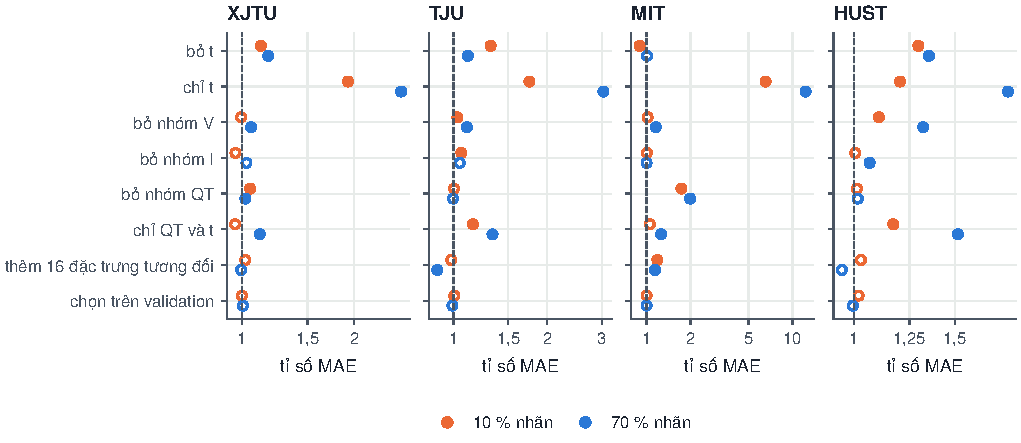
\includegraphics[width=\textwidth]{graphics/fig_features.pdf}
\caption[Bỏ hoặc thêm nhóm đầu vào: tỉ số MAE so với đủ 17 đầu vào]{Tỉ số MAE theo cell so với GBDT đủ 17 đầu vào, theo tập đầu vào và mức nhãn (thang log). Điểm đặc: khác có ý nghĩa (Wilcoxon theo cell, Holm qua bốn bộ); điểm rỗng: không có ý nghĩa. Vạch đứt: bằng bộ đầy đủ.}\label{fig:features}
\end{figure}


\subsection{Các đặc trưng và cách biến đổi đã bỏ}\label{sec:dt_bo}

Bảng~\ref{tab:dropped} tóm tắt những gì đã thử và bỏ. Ba dạng đầu là rò rỉ: chúng làm sai số đo được khác sai số thật khi triển khai, theo cả hai chiều tuỳ bộ (Bảng~\ref{tab:leak}), nên bị loại dù trên một số bộ chúng làm con số đẹp hơn. Đặc trưng tương đối bị loại ở bước chọn hướng cải tiến của PINN-lai vì làm sai số validation của PINN-semi tăng (tỉ số 1,692); phép chia cho mức ban đầu của cell khuếch đại các đặc trưng có giá trị ban đầu gần 0. Với GBDT, tác động của chúng trái chiều giữa các bộ (thấp hơn có ý nghĩa ở TJU 70\,\%, cao hơn có ý nghĩa ở MIT với cả hai mức nhãn), nên không dùng làm mặc định cho mọi bộ. Đặc trưng có lịch sử (Bảng~\ref{tab:hist} ở \Cref{sec:e20res}) giúp trên TJU và HUST khi có từ 30\,\% nhãn nhưng làm kém đi trên XJTU và ở 10\,\% nhãn, khi số chiều đầu vào tăng gấp đôi tới gấp bốn mà chỉ còn vài cell có nhãn; vì vậy PINN-lai không dùng chúng, còn HiPINN-lai chỉ dùng chúng ở các trường hợp validation chọn (\Cref{sec:pinnlai}, phân tích hậu kiểm). Nhiệt độ là hằng số trên ba bộ nên không mang thông tin; trên TJU, thêm $1/T$ vào GBDT cho tỉ số 0{,}99 (có ý nghĩa) ở 10\,\%, 1{,}00 ở 70\,\%, tức thay đổi dưới 1\,\%, nên nhiệt độ chỉ được giữ trong thừa số Arrhenius của động học. Đặc trưng từ lần xả và dung lượng các chu kỳ trước bị loại khỏi bài toán ước lượng vì đó chính là nhãn.

\begin{table}[!htbp]\centering\small
\caption[Các đặc trưng và cách biến đổi đã thử và bỏ]{Các đặc trưng và cách biến đổi đầu vào đã thử và bỏ, lý do và số liệu. Tỉ số là MAE so với cấu hình được dùng (lớn hơn 1: kém hơn; nhỏ hơn 1 ở hai hàng đầu: sai số trông thấp hơn thực tế vì rò rỉ).}\label{tab:dropped}
\begin{tabularx}{\textwidth}{>{\raggedright}p{3.6cm}>{\raggedright}p{4.2cm}>{\raggedright\arraybackslash}X}\toprule
Đã thử & Lý do bỏ & Số liệu \\\midrule
Chuẩn hoá min--max đặc trưng và $t$ theo cả vòng đời từng cell (như PINN4SOH) & dùng điểm cuối đời của cell, không có khi triển khai; $t$ sau chuẩn hoá là phần đời đã qua & MLP, 70\,\% nhãn: tỉ số XJTU 0{,}80, TJU 1{,}51, MIT 2{,}76, HUST 0{,}46 (Bảng~\ref{tab:leak}) \\
Lọc ngoại lai $3\sigma$ theo cả vòng đời, trên cả cột dung lượng & dùng tương lai của cell và cả nhãn & tỉ số 0{,}87--1{,}01 \\
Chuẩn hoá đặc trưng gồm cả cell test & dùng thống kê của tập test & tỉ số 0{,}98--1{,}03 \\
16 đặc trưng tương đối so với 3 chu kỳ đầu của cell & làm sai số validation của PINN-semi tăng; với GBDT tác động trái chiều giữa các bộ & PINN-semi, validation: tỉ số 1{,}692 (HUST 10\,\% nhãn: gấp 3{,}4 lần); GBDT, test: 0{,}89--1{,}19, cao hơn có ý nghĩa ở MIT với cả hai mức nhãn, thấp hơn có ý nghĩa ở TJU 70\,\% \\
Đặc trưng có lịch sử của cell (trung bình trượt mũ, độ dốc) & chỉ có lợi ở một số bộ khi đủ nhãn & Bảng~\ref{tab:hist}: PINN-lai 0{,}89--0{,}97 trên TJU, HUST từ 30\,\% nhãn; kém hơn trên XJTU (1{,}02--1{,}25); ở 10\,\% nhãn không giúp có ý nghĩa \\
Nhiệt độ làm đầu vào của mô hình & hằng số trên XJTU, MIT, HUST; trên TJU chỉ thay đổi sai số dưới 1\,\% & GBDT, TJU, thêm $1/T$: tỉ số 0{,}99$^{*}$ ở 10\,\%, 1{,}00 ở 70\,\% \\
Đặc trưng lấy từ lần xả, hoặc dung lượng đo của các chu kỳ trước & lần xả đầy chính là phép đo nhãn; khi ước lượng, dùng chúng là rò rỉ nhãn & chép nhãn chu kỳ gần nhất có sai số 0{,}01--0{,}15 lần mô hình thật (Bảng~\ref{tab:leak}); khi có đo thì dùng ở bước cập nhật (Mục~\ref{sec:budgetres}) \\
Đặc trưng cần đường cong thô (dung lượng gia tăng, điện áp hồi phục) & bản dữ liệu đã trích đặc trưng không có đường cong thô; chưa xử lý dữ liệu thô của từng bộ & chưa thử \\
\bottomrule\end{tabularx}\end{table}


\subsection{Kết luận về đầu vào}\label{sec:dt_ketluan}

Từ các kết quả trên, đồ án dùng đủ 16 đặc trưng đoạn sạc và $t = n/1000$: cả 17 tính được ở mọi chu kỳ từ dữ liệu sạc, 6 trên 6 tập rút gọn kém hơn có ý nghĩa ở ít nhất một trường hợp, không tập nào tốt hơn ở mọi bộ, và chọn bớt đặc trưng trên validation cho tỉ số 0{,}99--1{,}02. Đồ án không chuẩn hoá theo cả vòng đời cell, không lọc ngoại lai bằng tương lai của cell và không fit normaliser trên cell test, vì đây là rò rỉ và tác động của chúng lên sai số lên tới 0{,}46--2{,}76 lần tuỳ bộ. Đặc trưng tương đối không được dùng vì tác động trái chiều giữa các bộ; đặc trưng có lịch sử chỉ dùng khi validation chọn; nhiệt độ chỉ đi vào thừa số Arrhenius, vì thêm vào đầu vào chỉ thay đổi sai số dưới 1\,\%; thông tin của lần xả không được dùng khi ước lượng.



\section{Phương pháp}\label{ch:thuchien}

Mục này mô tả những gì đồ án xây dựng: giao thức đánh giá không rò rỉ, PINN-semi (PINN bán giám sát), mô hình kết hợp
PINN-lai, các mô hình đối chứng và các phần mở rộng.

\subsection{Giao thức đánh giá không rò rỉ}\label{sec:protocol}

Đơn vị chia dữ liệu là cell. Các chu kỳ liên tiếp của một cell gần như giống nhau, nên nếu chia ngẫu nhiên theo chu kỳ,
gần như mọi chu kỳ kiểm tra đều có một chu kỳ kề bên trong tập huấn luyện. Mệnh đề dưới đây lượng hoá điều này.

\begin{menhde}[Cận sai số khi chia theo chu kỳ]\label{md:rowleak}
Giả sử mỗi chu kỳ được đưa vào tập huấn luyện độc lập với xác suất $q$. Xét bộ dự đoán không dùng đặc trưng nào, chỉ chép
nhãn của chu kỳ huấn luyện gần nhất trong cùng cell. Bỏ qua hiệu ứng ở hai đầu cell, khoảng cách $d$ tới chu kỳ huấn
luyện gần nhất thoả $\E[d] = 1/(1 - (1-q)^2)$, và sai số tuyệt đối kỳ vọng không vượt quá $\E[d]\cdot\overline{|\Delta
y|}$, với $\overline{|\Delta y|}$ là biến thiên nhãn trung bình giữa hai chu kỳ liền kề.
\end{menhde}
\begin{proof}
$d > j$ khi và chỉ khi $2j$ chu kỳ gần nhất về hai phía đều không thuộc tập huấn luyện, với xác suất $(1-q)^{2j}$, nên
$\E[d] = \sum_{j \ge 0} P(d > j) = 1/(1-(1-q)^2)$. Theo bất đẳng thức tam giác, sai số chép nhãn không vượt tổng $d$
biến thiên liền kề dọc quỹ đạo từ chu kỳ kiểm tra tới chu kỳ huấn luyện gần nhất. Lấy kỳ vọng được
$\sum_{i \ge 0} P(d > i)\,\overline{|\Delta y|} = \E[d]\cdot\overline{|\Delta y|}$.
\end{proof}
Với $q = 0{,}7$, $\E[d] = 1{,}099$ chu kỳ, nên một mô hình đánh giá theo cách chia này có thể đạt sai số rất thấp chỉ bằng
cách nhớ quỹ đạo. Vì vậy đồ án chia theo cell: mọi chu kỳ của một cell nằm trọn trong tập huấn luyện, tập xác thực hoặc
tập kiểm tra.

Đồ án dùng kiểm định chéo 5 fold theo cell. Trong mỗi fold, 20\,\% số cell làm tập kiểm tra, 10\,\% làm tập xác thực (để
dừng sớm và chọn siêu tham số), và 70\,\% còn lại làm tập huấn luyện. Với cách chia này, tập huấn luyện vừa đủ chứa mức
nhãn cao nhất 70\,\%, còn bộ nhỏ nhất (XJTU) vẫn có 11 cell kiểm tra và 6 cell xác thực mỗi fold. Cách chia được phân tầng
theo chế độ thí nghiệm: trong mỗi chế độ, cell được xáo rồi chia vòng tròn với một bộ đếm chạy tiếp qua các chế độ. Nhờ
vậy mỗi cell được kiểm tra đúng một lần ở mỗi lần lặp, và số cell của một chế độ trong các fold lệch nhau không quá 1.
Toàn bộ được lặp 5 lần với 5 cách xáo khác nhau. Một số thí nghiệm về sau dùng 3 lần lặp đầu.

Có bốn mức nhãn: 10, 30, 50 và 70\,\% số cell của bộ có nhãn, chọn từ các cell huấn luyện theo một thứ tự vòng tròn cố
định qua các chế độ. Tập có nhãn ở mức thấp là tập con của tập ở mức cao, nên khi tăng mức nhãn, khác biệt duy nhất là có
thêm nhãn. Ở fold $k$ của lần lặp $r$, mọi mô hình dùng chung hạt giống $100r + k$, tức cùng cell huấn luyện, cùng cell
có nhãn, cùng cell xác thực và cùng cell kiểm tra, nên các mô hình so được với nhau theo từng cell.

Bốn quy tắc chống rò rỉ được cài sẵn trong mã. Thứ nhất, bộ chuẩn hoá chỉ được fit trên đặc trưng của cell huấn luyện.
Thứ hai, bộ lọc ngoại lai quyết định giữ hay bỏ chu kỳ $n$ chỉ bằng các chu kỳ trước $n$ của chính cell. Thứ ba, biến
thời gian $t = n/1000$ dùng một hằng số chung. Thứ tư, mọi tham số học và mọi lựa chọn trong một fold, như dừng sớm, số
cây, trọng số ghép hay cửa sổ lọc, chỉ dựa trên cell xác thực của chính fold đó. Tập kiểm tra chỉ dùng một lần để đánh
giá. Thang đời $L$ dùng để đặt lịch đo ở các phần mở rộng cũng chỉ tính trên cell huấn luyện của fold. Có một ngoại lệ
được nêu rõ: ở giai đoạn phát triển, một số lựa chọn rời rạc (thành phần của PINN-lai, dạng đặc trưng lịch sử, độ dài cửa
sổ của mô hình chuỗi) được chốt trên tập xác thực của lần lặp 0 gộp qua 5 fold. Mỗi cell vì vậy có thể đã góp vào các lựa
chọn này khi nó là cell xác thực ở một fold khác. Các lựa chọn này được chốt trước khi đọc bất kỳ dự đoán nào trên tập
kiểm tra.

\subsection{Mô hình PINN bán giám sát}\label{sec:pinn}

Mô hình gồm hai mạng nối với nhau qua hàm mất mát (Hình~\ref{fig:arch}). Mạng nghiệm $F_\varphi$ dự đoán SOH, còn mạng
tốc độ $G_\theta$ cùng hai tham số vật lý $\lambda, E_a$ mô tả tốc độ suy giảm. Khi suy luận chỉ cần $F_\varphi$.

\begin{figure}[!htbp]\centering
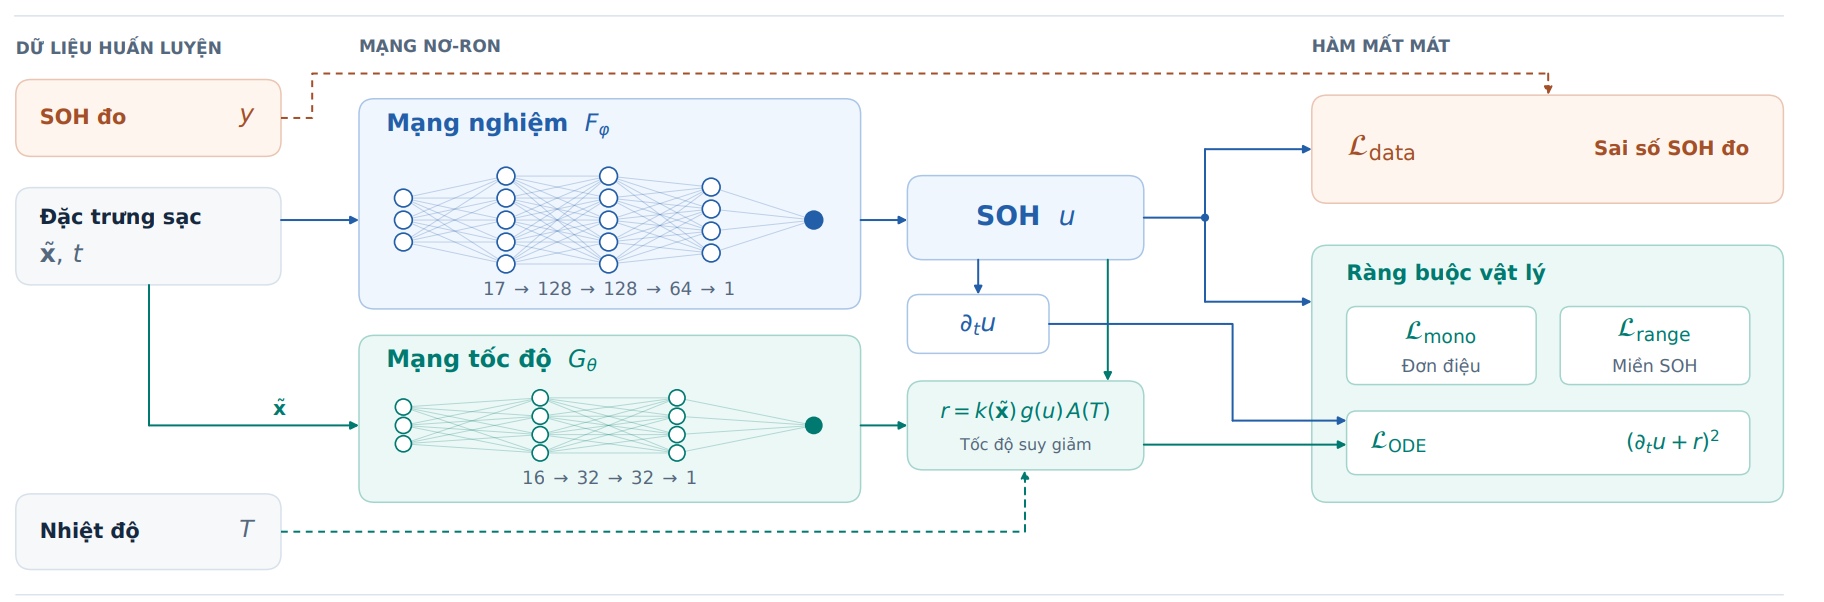
\includegraphics[width=\textwidth]{graphics/fig_pinn_semi.png}
\caption[Kiến trúc PINN bán giám sát]{Kiến trúc PINN bán giám sát: mạng nghiệm $F_\varphi$ dự đoán SOH $u$ từ đặc trưng
sạc và $t$; mạng tốc độ $G_\theta$ cùng nhiệt độ $T$ cho tốc độ suy giảm $r = k(\tilde{\mathbf{x}})\,g(u)\,A(T)$.
$\mathcal{L}_\text{data}$ chỉ tính trên chu kỳ có nhãn, ba ràng buộc vật lý tính trên mọi cell.}\label{fig:arch}
\end{figure}

Mạng nghiệm $u = F_\varphi(\tilde{\mathbf{x}}, t)$ là perceptron 17--128--128--64--1 với hàm kích hoạt SiLU. Tốc độ suy
giảm có dạng xám:
\begin{equation}\label{eq:rate}
r(\tilde{\mathbf{x}}, u, T) =
\underbrace{\operatorname{softplus}\big(G_\theta(\tilde{\mathbf{x}})\big)}_{k(\mathbf{x})}\;
\underbrace{e^{\lambda\,\operatorname{clip}(1-u,\,-0{,}5,\,1)}}_{g(u)}\;
\underbrace{e^{-\frac{E_a}{R_g}\left(\frac{1}{T}-\frac{1}{T_\text{ref}}\right)}}_{A(T)},
\qquad \frac{\partial u}{\partial t} = -\,r(\tilde{\mathbf{x}}, u, T),
\end{equation}
với $G_\theta$ là perceptron 16--32--32--1, $\lambda = \operatorname{softplus}(\lambda_\text{raw})$,
$E_a = 10^4 \operatorname{softplus}(e_\text{raw})$\,J/mol và $T_\text{ref} = 298{,}15$\,K. Thừa số $k$ là tốc độ cơ sở
phụ thuộc trạng thái điện hoá (đọc qua đặc trưng sạc), $g$ làm suy giảm tăng nhanh khi SOH thấp, còn $A$ là hệ số
Arrhenius. Vì softplus và hàm mũ đều dương, $r \ge 0$ với mọi tham số, nên mọi nghiệm của phương trình không tăng theo
$t$. Tính chất này đúng theo $t$ khi giữ $\tilde{\mathbf{x}}$ cố định. Trên quỹ đạo thật của một cell, đặc trưng sạc đổi
theo chu kỳ, nên SOH ước lượng không bị buộc phải giảm đơn điệu mà chỉ được khuyến khích giảm bởi $\mathcal{L}_\text{mono}$
dưới đây. Khi nhiệt độ của một bộ dữ liệu không đổi, $A(T)$ chỉ là một hằng số nhân và bị $k$ hấp thụ, nên $E_a$ không
xác định được từ dữ liệu của bộ đó (\Cref{sec:vatly}).

Hàm mất mát dùng các cặp chu kỳ $(n_1, n_2)$ của cùng cell với $n_2 \ge n_1 + h$, $h \sim \mathcal{U}\{5, \dots, 50\}$, và
$u_i = F_\varphi(\tilde{\mathbf{x}}_{n_i}, t_{n_i})$:
\begin{align}
\mathcal{L}_\text{data} &= \tfrac{1}{B}\textstyle\sum (u - y)^2 && \text{(chỉ chu kỳ có nhãn)},\\
\mathcal{L}_\text{ode} &= \tfrac{1}{B}\textstyle\sum \big(\partial_t u_1 + r(\tilde{\mathbf{x}}_{n_1}, u_1, T)\big)^2, \\
\mathcal{L}_\text{mono} &= \tfrac{1}{B}\textstyle\sum \operatorname{ReLU}(u_2 - u_1 - \varepsilon), && \varepsilon = 0{,}002,\\
\mathcal{L}_\text{range} &= \tfrac{1}{B}\textstyle\sum \big[\operatorname{ReLU}(u_1 - 1{,}15) + \operatorname{ReLU}(0{,}4 - u_1)\big],
\end{align}
cộng một ràng buộc giữ SOH ở chu kỳ đầu của cell trong $[0{,}85;\,1{,}10]$. Hàm mất mát toàn phần là
\begin{equation}
\mathcal{L} = \mathcal{L}_\text{data} + w(s)\big(\alpha\mathcal{L}_\text{ode} + \beta\mathcal{L}_\text{mono}
+ \gamma\mathcal{L}_\text{range}\big), \qquad w(s) = \min\big(1, s/(0{,}2S)\big),
\end{equation}
với $\alpha = 0{,}02$, $\beta = 0{,}5$, $\gamma = 1$ và $S = 4000$ bước. Đạo hàm $\partial_t u$ tính bằng vi phân tự động.
Trọng số $w(s)$ tăng dần trong 20\,\% số bước đầu để mạng học nhãn trước khi chịu ràng buộc vật lý đầy đủ.

Cơ chế bán giám sát nằm ở cách lấy mẫu: một nửa số cặp chu kỳ lấy từ cell có nhãn, một nửa từ cell không nhãn. Ba hàm
mất mát vật lý không chứa $y$, chỉ phụ thuộc đặc trưng, thời điểm, nhiệt độ và tham số mô hình, nên tính được trên mọi cell
chỉ có dữ liệu sạc. Mạng nghiệm vì vậy bị buộc cho quỹ đạo hợp lý vật lý trên chính những cell mà nó phải tổng quát tới.
Khác với PINN4SOH, tốc độ $r$ không nhận $u_t$ làm đầu vào và luôn không âm, nên phần dư động học không thể được thoả
mãn một cách tầm thường bằng $G \approx u_t$.

\subsection{Mô hình kết hợp PINN-lai}\label{sec:pinnlai}

PINN-lai gồm ba bước (\Cref{fig:pinnlai}):
\begin{align}
\bar F(\mathbf{x}, t) &= \tfrac{1}{3}\textstyle\sum_{m=1}^{3} F_{\varphi_m}(\tilde{\mathbf{x}}, t), \\
\hat y_n &= \omega\,\bar F(\mathbf{x}_n, t_n) + (1 - \omega)\,g(\mathbf{x}_n, t_n), \\
\tilde y_n &= \bar y + \min(0, \hat\beta)\,(t_n - \bar t) \quad \text{trên cửa sổ } \hat y_{n-w+1}, \dots, \hat y_n,
\end{align}
với $F_{\varphi_m}$ là ba PINN-semi chỉ khác hạt giống và $g$ là GBDT học trên cùng các cell có nhãn. Bước cuối khớp một
đường thẳng có độ dốc không dương lên $w$ ước lượng gần nhất của chính cell rồi lấy giá trị tại chu kỳ hiện tại, gọi là
bộ lọc xu thế nhân quả~\cite{cleveland1979}. Bộ lọc không làm lệch một quỹ đạo giảm tuyến tính, và với nhiễu độc lập
phương sai $\sigma^2$, nó giảm phương sai còn $0{,}345\,\sigma^2$ khi $w = 10$.

PINN-lai dùng cấu hình cố định $\omega = \tfrac12$ và $w = 10$. Cấu hình này được chọn trong 9 hướng cải tiến ở giai đoạn
phát triển, chỉ bằng tập xác thực của lần lặp 0 (Mục~\ref{sec:e20res}), và được ấn định trước khi đọc bất kỳ dự đoán nào
trên tập kiểm tra. Sau khi có kết quả của bản cố định, đồ án thử thêm một bản tinh chỉnh: $(\omega, w)$ được chọn trên
lưới $\omega \in \{0{,}3; 0{,}4; 0{,}5; 0{,}6; 0{,}7\}$, $w \in \{5, 10, 20, 40\}$ riêng cho từng fold, chỉ bằng MAE trên
cell xác thực của fold đó. Vì ý tưởng tinh chỉnh có sau khi đã xem kết quả kiểm tra của bản cố định, bản tinh chỉnh chỉ
được nêu để đối chiếu. Mọi kết quả khác của báo cáo dùng PINN-lai cố định.

\begin{figure}[!htbp]\centering
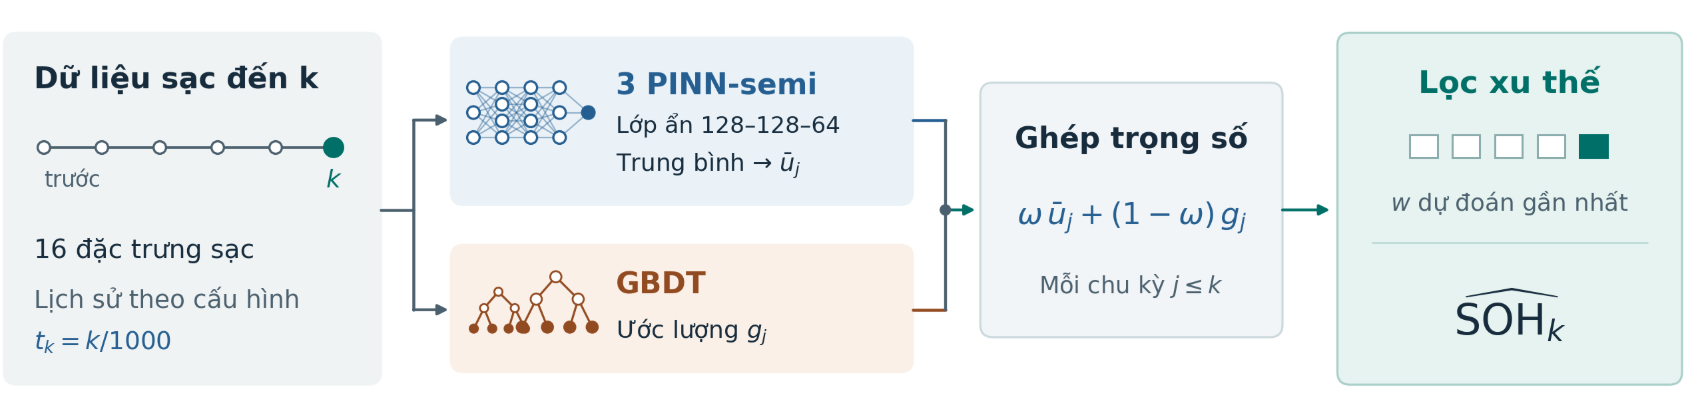
\includegraphics[width=\textwidth]{graphics/fig_pinn_lai.png}
\caption[PINN-lai và HiPINN-lai]{PINN-lai và HiPINN-lai: ba PINN-semi và GBDT ước lượng SOH ở từng chu kỳ $j \le k$,
ghép theo trọng số $\omega$, rồi lọc xu thế trên $w$ ước lượng gần nhất. HiPINN-lai thêm đặc trưng lịch sử của đặc trưng
sạc, chỉ ở những fold mà tập xác thực chọn.}\label{fig:pinnlai}
\end{figure}

HiPINN-lai (History-informed PINN-lai) là PINN-lai có thêm lịch sử của cell trong đầu vào. Ngoài đặc trưng sạc
$\mathbf{x}_n$ của chu kỳ hiện tại, mô hình nhận các đại lượng chỉ dùng chu kỳ $n$ và các chu kỳ trước của chính cell, nên
vẫn chạy trực tuyến được. Đó là trung bình trượt mũ $\mathbf{z}^{(a)}_n = a\,\mathbf{x}_n + (1-a)\,\mathbf{z}^{(a)}_{n-1}$,
nhớ khoảng $1/a$ chu kỳ, với $a \in \{0{,}3;\ 0{,}1;\ 0{,}03\}$, và độ dốc bình phương tối thiểu của từng đặc trưng trên 20
chu kỳ gần nhất. Lịch sử ở đây là lịch sử của đặc trưng sạc, không phải của SOH, vì cell cần ước lượng không được đo dung
lượng. Đây là điểm khác với HiGBDT và HiPINN ở bài toán dự báo (\Cref{sec:e33pp}), vốn dùng lịch sử SOH đo. Dạng lịch sử
của mỗi bộ được chốt ở giai đoạn phát triển trên tập xác thực của lần lặp 0. Ba PINN-semi và GBDT có lịch sử được ghép
đúng như PINN-lai cố định. Trong từng fold, HiPINN-lai dùng bản có lịch sử nếu MAE trên cell xác thực của fold đó thấp hơn
PINN-lai ít nhất 2\,\%, nếu không thì nó trùng PINN-lai. Vì vậy trên bộ không có dạng lịch sử nào được chọn, HiPINN-lai
trùng PINN-lai ở mọi fold. Kết quả của HiPINN-lai là phân tích hậu kiểm (\Cref{sec:e20res}).

\subsection{Mô hình đối chứng và cấu hình huấn luyện}\label{sec:baselines}

Mọi mô hình ở Bảng~\ref{tab:models} dùng cùng đầu vào, cùng cách chia, cùng tập cell có nhãn và cùng bộ chuẩn hoá.

\begin{table}[!htbp]\centering\small
\caption{Các mô hình được so sánh.}\label{tab:models}
\begin{tabularx}{\textwidth}{l>{\raggedright}p{3.2cm}>{\raggedright\arraybackslash}X}
\toprule
Mô hình & Nhóm & Mô tả \\
\midrule
Ridge & học có nhãn & hồi quy tuyến tính chuẩn hoá $L_2$; $\alpha \in \{10^{-3},\dots,10^{3}\}$ chọn trên tập xác thực\\
GPR & học có nhãn & nhân RBF + nhiễu trắng, 1\,500 điểm có nhãn chọn ngẫu nhiên\\
GBDT & học có nhãn & dạng histogram, tốc độ học 0,05, 31 lá; số cây $\le 1000$ chọn trên tập xác thực\\
MLP & học có nhãn & cùng kiến trúc với mạng nghiệm, chỉ $\mathcal{L}_\text{data}$\\
CNN & học có nhãn, chuỗi & tích chập nhân quả, 32 kênh, kích thước 5, độ giãn 1 và 2, cửa sổ 16 chu kỳ\\
LSTM & học có nhãn, chuỗi & một lớp 32 nút ẩn, cửa sổ 48 chu kỳ\\
Transformer & học có nhãn, chuỗi & một lớp mã hoá 32 chiều, 4 đầu chú ý, mã hoá vị trí hình sin, cửa sổ 16 chu kỳ\\
PINN-sup & vật lý trên cell có nhãn & như PINN-semi nhưng hàm mất mát vật lý chỉ tính trên cell có nhãn\\
PINN hộp đen & vật lý, bán giám sát & động học kiểu PINN4SOH, $u_t = G(\mathbf{x}, t, u, u_\mathbf{x}, u_t)$, cùng các hàm
mất mát không nhãn\\
PINN-semi & vật lý, bán giám sát & mô hình đề xuất\\
PINN-lai & kết hợp & ba PINN-semi, GBDT, bộ lọc xu thế; $\omega = \tfrac12$, $w = 10$\\
\bottomrule
\end{tabularx}
\end{table}

MLP và các biến thể PINN dùng AdamW~\cite{loshchilov2019} với tốc độ học $2\cdot10^{-3}$ giảm theo cosine về $10^{-4}$
trong 4\,000 bước. Mỗi lô (batch) gồm 512 điểm có nhãn và 512 cặp chu kỳ. Gradient được cắt ở chuẩn 5, và việc dừng sớm
theo MAE trên tập xác thực. Độ dài cửa sổ của CNN, LSTM và Transformer được chọn trong $\{16, 48\}$ trên tập xác thực.
Trọng số vật lý được chọn trước ở một thí nghiệm sơ bộ và giữ cố định. Không siêu tham số nào được chọn theo tập kiểm tra.

\subsection{Ngân sách đo và cập nhật khi dùng}\label{sec:mo_rong}

Phần mở rộng thứ nhất thay đổi cách gắn nhãn khi huấn luyện. Thay vì đo đầy đủ một phần cell, mọi cell huấn luyện được đo
dung lượng ở chu kỳ đầu, sau mỗi $qL$ chu kỳ và ở chu kỳ cuối, với $q \in \{0{,}5;\ 0{,}2;\ 0{,}1;\ 0{,}05\}$ và $L$ là trung
vị số chu kỳ của các cell huấn luyện của fold. PINN-semi chỉ tính $\mathcal{L}_\text{data}$ trên các chu kỳ được đo, còn
hàm mất mát vật lý vẫn tính trên mọi hàng. GBDT học nhãn nội suy tuyến tính giữa các lần đo.

Phần mở rộng thứ hai xét lúc dùng, khi cell mới cũng được đo dung lượng vài lần. Cách thứ nhất là bộ lọc Kalman ở
\Cref{sec:lt_kalman}: sai số $y_n - p_n$ giữa SOH đo và SOH ước lượng được mô hình hoá bằng một độ lệch trôi chậm hồi quy
về trung bình cộng nhiễu, và được cập nhật mỗi khi có một lần đo. Bốn tham số của bộ lọc được ước lượng trên cell xác thực
của từng fold. Cách thứ hai là GBDT-cập nhật, một GBDT học thẳng SOH đã đổi bao nhiêu kể từ lần đo gần nhất. Trong cả hai
cách, lịch đo của cell kiểm tra (chu kỳ đầu rồi mỗi $qL$ chu kỳ) dùng $L$ tính trên cell huấn luyện của fold. HiGBDT ở mục
sau cũng được áp dụng cho bài toán này (\Cref{sec:anchor}).

\subsection{Dự báo SOH, dung lượng và RUL: HiGBDT và HiPINN}\label{sec:e33pp}

Bài toán dự báo được đặt như sau. Đứng ở chu kỳ gốc $k$ của một cell, ta biết đặc trưng sạc của mọi chu kỳ tới $k$ và SOH
đo được tới $k$ (dung lượng đo chia dung lượng danh định), và cần dự báo SOH ở mọi chu kỳ $k+h$ sau đó. Dung lượng là SOH
nhân dung lượng danh định. RUL là số chu kỳ tới khi SOH xuống dưới ngưỡng cuối đời $\tau$ của bộ (\Cref{tab:fcset}). Đồ án
xây dựng hai mô hình có đặc trưng lịch sử: HiGBDT (History-informed GBDT), một GBDT có đặc trưng lịch sử SOH, và HiPINN
(History-informed PINN), trung vị của ba nhánh (\Cref{fig:hipinntq}). Phần dưới mô tả trước các khối dùng chung, rồi tới
hai mô hình này.

\begin{figure}[!htbp]\centering
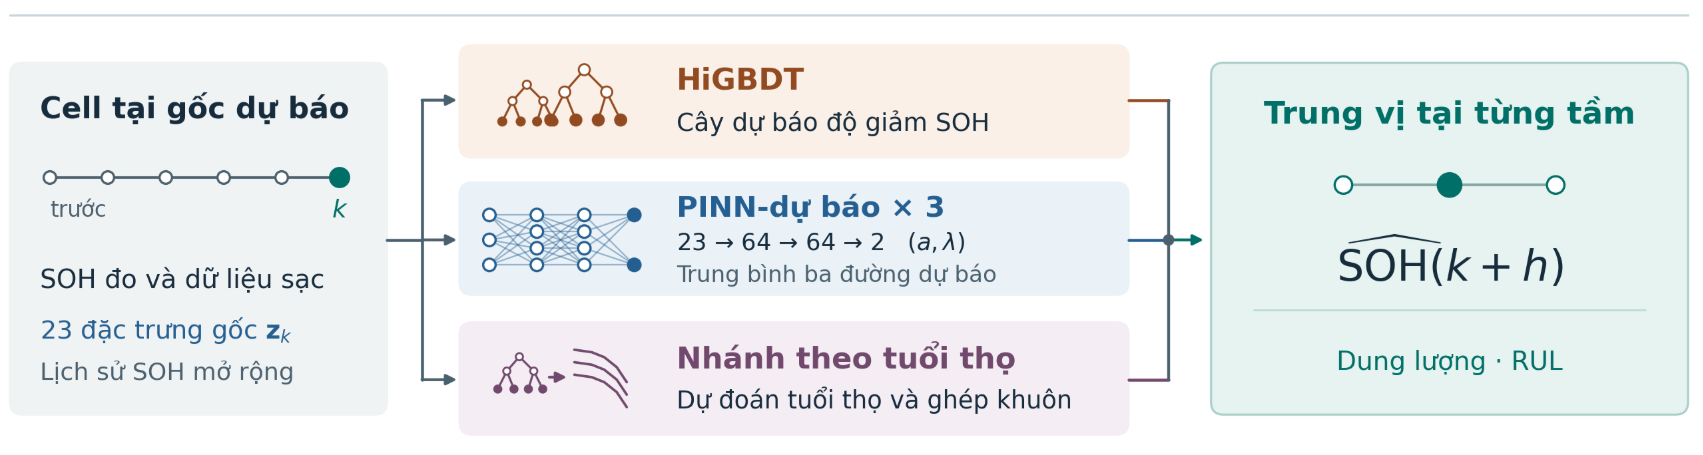
\includegraphics[width=\textwidth]{graphics/fig_hipinn_tongquan.png}
\caption[Tổng quan HiPINN]{Tổng quan HiPINN: tại gốc $k$, từ SOH đo và dữ liệu sạc của cell, ba nhánh HiGBDT, PINN-dự
báo (ba mạng) và nhánh theo đời (dự đoán tuổi thọ rồi ghép khuôn quỹ đạo) cùng dự báo SOH; trung vị tại từng tầm cho
$\widehat{\mathrm{SOH}}(k+h)$, dung lượng và RUL.}\label{fig:hipinntq}
\end{figure}

\begin{table}[!htbp]\centering\small
\caption[Tham số đánh giá dự báo của từng bộ]{Tham số đánh giá dự báo của từng bộ: $L$ là trung vị số chu kỳ ghi được của mọi cell trong bộ (khi học, $L$ tính lại trên cell huấn luyện của từng fold), $\tau$ là ngưỡng cuối đời.}\label{tab:fcset}
\begin{adjustbox}{max width=\textwidth}\begin{tabular}{lrrrrr}\toprule
Bộ & Số cell & $L$ (chu kỳ) & $\tau$ & Cell có chu kỳ cuối đời & $C_\text{dđ}$ (Ah) \\\midrule
XJTU & 55 & 392 & 0{,}84 & 78\,\% & 2{,}0 \\
TJU & 130 & 377 & 0{,}81 & 79\,\% & 2{,}5--3{,}5 \\
MIT & 125 & 622 & 0{,}87 & 81\,\% & 1{,}1 \\
HUST & 77 & 1855 & 0{,}81 & 96\,\% & 1{,}1 \\
\bottomrule\end{tabular}\end{adjustbox}\end{table}


Ngưỡng cuối đời $\tau$ không lấy chung 0,8 như quy ước xe điện ở \Cref{sec:bai_toan}, vì nhiều cell trong các thí nghiệm này dừng thử trước khi SOH xuống 0,8. Tỉ lệ cell có SOH đo chạm 0,8 chỉ là 36\,\% ở XJTU, 77\,\% ở TJU, 0\,\% ở MIT và 8\,\% ở HUST, nên RUL theo ngưỡng 0,8 không xác định được cho phần lớn cell. Với mỗi bộ, $\tau$ được chọn trước khi học mô hình theo một quy tắc chỉ dựa trên phạm vi dữ liệu: mức thấp nhất trên lưới bước 0,01 mà ít nhất 80\,\% số cell của bộ có SOH đo chạm tới. Quy tắc này cho $\tau$ = 0{,}84 (XJTU), 0{,}81 (TJU), 0{,}87 (MIT) và 0{,}81 (HUST). Quy tắc dùng SOH đo của mọi cell trong bộ, kể cả cell kiểm tra, nhưng chỉ để định nghĩa mục tiêu RUL chung cho mọi mô hình, không thay đổi đầu vào hay tham số của mô hình nào. Cột ``cell có chu kỳ cuối đời'' của \Cref{tab:fcset} đếm theo định nghĩa chặt hơn dùng khi chấm, tức trung vị trượt 9 chu kỳ của SOH đo xuống dưới $\tau$, nên có bộ thấp hơn 80\,\% một chút. Vì $\tau$ khác nhau giữa các bộ, RUL của các bộ không so trực tiếp với nhau.


Các mô hình dự báo dùng chung một vectơ đặc trưng gốc $\mathbf{z}_k$ gồm 23 giá trị tính từ lịch sử tới $k$: mức SOH hiện
tại $\ell_k$ (xu thế nhân quả trên 10 hàng), độ dốc bình phương tối thiểu trên 30 và 100 hàng gần nhất, mức ban đầu
$\ell_0$ và độ giảm $\ell_0 - \ell_k$, $k$, $1/T$, và trung bình 16 đặc trưng sạc đã chuẩn hoá trên 10 hàng gần nhất.
PINN-dự báo là một mạng nhỏ hai lớp ẩn 64 nút, nhận $\mathbf{z}_k$ và trả hai tham số $(a, \lambda)$ của nghiệm đóng của
động học xám $dv/dN = a_0 e^{\lambda v}$, với $v = 1 - \text{SOH}$, khi coi tốc độ cơ sở là hằng trong tầm dự báo:
\begin{equation}\label{eq:fcdrop}
\hat y(k+h) = \ell_k + \frac{1}{\lambda}\ln\bigl(1 - \lambda a h\bigr),
\end{equation}
với $a \geq 0$ là tốc độ suy giảm tại $k$. Đường dự báo luôn không tăng. Nó giảm nhanh dần khi $\lambda > 0$ (đầu gối) và
chậm dần khi $\lambda < 0$. Ba mạng với hạt giống khác nhau được lấy trung bình. GBDT theo tầm học trực tiếp độ giảm
$\ell_k - \text{SOH}(k+h)$ từ $(\mathbf{z}_k, h)$, có ràng buộc đơn điệu tăng theo $h$. PINN-GBDT lấy trung bình hai mô
hình này với trọng số bằng nhau. Ba mô hình này chỉ nhìn lịch sử của cell qua mức SOH và hai độ dốc trong $\mathbf{z}_k$,
và được giữ làm mốc so sánh. Mọi mô hình học trên các mẫu (gốc, tầm) lấy từ lịch sử đo thật của cell huấn luyện, 40 gốc
và 40 tầm mỗi cell. Số cây của GBDT và điểm dừng của PINN-dự báo được chọn theo MAE trên cell xác thực.

Đồ án thiết kế HiGBDT để vừa là một mô hình dự báo đứng riêng, vừa là một nhánh của HiPINN. Ngoài 23 đặc trưng gốc
$\mathbf{z}_k$, HiGBDT nhận SOH tại $k$ và độ lệch của nó so với mức $\ell_k$. Với các cửa sổ 5, 10, 30, 100 và 200 hàng
gần nhất, mô hình nhận trung bình trừ SOH hiện tại, độ lệch chuẩn và độ dốc. Với độ trễ 1, 3, 7, 15, 31 và 63 hàng, mô
hình nhận thay đổi SOH và khoảng chu kỳ tương ứng. Tất cả chỉ dùng các hàng tới gốc. GBDT học độ giảm $\ell_k -
\text{SOH}(k+h)$ theo (đặc trưng, $h$). Sáu cấu hình được thử: hàm mất mát $L_2$ hoặc $L_1$, 15 hoặc 31 lá, có hoặc không
ràng buộc đơn điệu theo $h$, học phần dư so với ngoại suy tuyến tính, và một cấu hình chỉ dùng 23 đặc trưng gốc để làm mốc.
Mỗi cấu hình có 100, 250 hoặc 450 cây. Cấu hình, số cây và trọng số $a \in \{0;\ 0{,}25;\ 0{,}5;\ 0{,}75;\ 1\}$ trộn với
GBDT theo tầm được chọn theo MAE trên tập xác thực. Khi học và khi chọn, mỗi cell và mỗi gốc có tổng trọng số như nhau,
để cell dài không lấn át cell ngắn.

Để trả lời câu hỏi lịch sử có giúp chính PINN-dự báo hay không, đồ án giữ nguyên mạng và nghiệm đóng~\eqref{eq:fcdrop}
nhưng đổi đầu vào thành 23 đặc trưng gốc cộng các đặc trưng lịch sử ở trên. Mô hình này gọi là PINN-dự báo có lịch sử.
Khi đó mạng và HiGBDT nhận cùng một lượng thông tin và chỉ khác dạng mô hình: cây quyết định học tự do theo $h$, còn mạng
chỉ chọn tham số cho một đường suy giảm có dạng vật lý. Mô hình này được so riêng, không nằm trong HiPINN.

Hai nhánh trên dự báo trực tiếp SOH tại $k+h$. Với các cell suy giảm chậm rồi gãy gần cuối đời, thời điểm gãy mỗi cell
một khác, nên dự báo trực tiếp có xu hướng thành một đường trung bình gần thẳng: thấp hơn thực tế ở giữa đời và cao hơn
thực tế ở phần cuối. Nhánh theo đời tách việc dự báo thành hai bước. Bước một, một GBDT học đời còn lại $\log(N_j - c)$
từ cùng bộ đặc trưng có lịch sử, với $N_j$ là chu kỳ mà SOH của cell huấn luyện $j$ chạm ngưỡng $\tau$. Cell chưa chạm
ngưỡng không được dùng. Bước hai, mỗi cell huấn luyện cho một khuôn $f_j(u) = \text{SOH}_j(u N_j)$ theo thời gian chuẩn
hoá $u$, làm trơn bằng trung vị trượt 9 hàng. Với đời dự đoán $\hat N = c_k + \widehat{N - c_k}$ của cell cần dự báo,
\begin{equation}\label{eq:life}
\hat y(c_k + h) = \ell_k + \frac{1}{K}\sum_{j \in \mathcal{K}}
  \Bigl[f_j\Bigl(\frac{c_k + h}{\hat N}\Bigr) - f_j\Bigl(\frac{c_k}{\hat N}\Bigr)\Bigr],
\end{equation}
trong đó $\mathcal{K}$ là $K$ khuôn có đặc trưng gốc gần nhất ở cùng thời điểm chuẩn hoá, hoặc mọi khuôn. Sau điểm cuối
của khuôn, giá trị cuối được giữ nguyên, vì trên tập xác thực, kéo dài khuôn theo độ dốc cuối đời làm dự báo sụp xuống mỗi
khi đời bị đoán ngắn đi nhiều. Số cây và $K \in \{5, 10, 20, \text{mọi khuôn}\}$ được chọn trên tập xác thực. Nhánh này
được thêm sau khi thấy sai số ở phần cuối đời trong lần chạy đầu của thí nghiệm dự báo (\Cref{sec:e33res}), nên kết quả
của nó là kết quả sau thí nghiệm.

HiPINN lấy trung vị của ba nhánh tại từng gốc và tầm:
\begin{equation}\label{eq:e33}
\hat y = \operatorname{med}\bigl(\hat y_\text{HiGBDT},\ \hat y_\text{PINN},\ \hat y_\text{theo đời}\bigr),
\end{equation}
trong đó nhánh PINN là PINN-dự báo chỉ với 23 đặc trưng gốc. Ba nhánh sai theo những cách khác nhau. PINN-dự báo có thể
lệch xa ở cell có đường suy giảm khác dạng nghiệm đóng, nhánh theo đời đặt sai điểm gãy khi đời bị đoán sai, còn HiGBDT
thường dự báo phần cuối đời cao hơn thực tế. Khi chỉ một nhánh sai xa, trung vị đi theo hai nhánh còn lại, trong khi trung
bình bị kéo về phía nhánh sai. Trung vị cũng không có tham số nào cần chọn.

Phương án đầu của HiPINN, gọi là HiPINN-w, là tổng có trọng số $w_1\hat y_\text{HiGBDT} + w_2\hat y_\text{PINN} +
w_3\hat y_\text{theo đời}$, với $(w_1, w_2, w_3)$ trên lưới bước 0,25 có tổng bằng 1 và nhánh PINN (có hoặc không có lịch
sử) chọn theo MAE trên nửa tập xác thực dùng để chọn. Nửa này chỉ gồm vài cell mỗi lượt, nên trọng số chọn được không giữ
được ưu thế trên nửa còn lại (\Cref{sec:e33res}). Vì vậy HiPINN dùng trung vị. Quyết định này đưa ra sau khi đã có kết quả
kiểm tra của phương án đầu, nên kết quả của HiPINN là kết quả sau thí nghiệm. HiPINN-w và HiPINN-tb, trung bình đều ba
nhánh, được giữ trong các bảng để đối chiếu. Khoảng 90\,\% của dự báo theo phương pháp conformal: $q$ là phân vị 90\,\% của
$|y - \hat y| / \sqrt{1 + h/L}$ trên các cell hiệu chỉnh, và khoảng là $\hat y \pm q\sqrt{1 + h/L}$.

\begin{figure}[!htbp]\centering
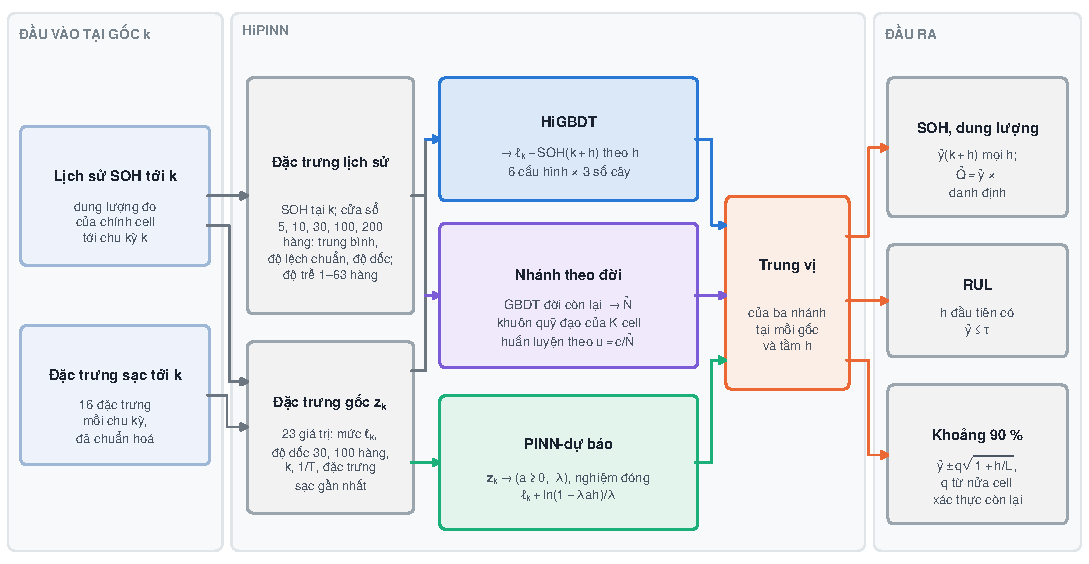
\includegraphics[width=\textwidth]{graphics/fig_hipinn_arch.pdf}
\caption[Chi tiết mô hình HiPINN]{Chi tiết HiPINN tại gốc $k$: HiGBDT và nhánh theo đời nhận đặc trưng gốc và đặc trưng
lịch sử SOH, PINN-dự báo nhận đặc trưng gốc; trung vị của ba nhánh cho SOH và dung lượng dự báo, RUL và khoảng
90\,\%.}\label{fig:hipinn}
\end{figure}

Dự báo dùng đúng các fold theo cell và các lần lặp của PINN-lai (5 fold, 70/10/20\,\% số cell cho tập huấn luyện, tập xác
thực và tập kiểm tra, ba lần lặp), nên mỗi cell được dự báo một lần ở mỗi lần lặp, bởi mô hình chưa thấy cell đó. Cell
xác thực được chia đôi theo thứ tự tên. Nửa thứ nhất, gọi là nửa chọn, dùng để chọn cấu hình, số cây, trọng số và điểm dừng.
Nửa thứ hai, gọi là nửa hiệu chỉnh, dùng để hiệu chỉnh khoảng và để so các mô hình trên những cell không dùng khi chọn. Thang đời $L$ (trung vị số
chu kỳ của cell huấn luyện) và bộ chuẩn hoá chỉ tính trên cell huấn luyện. Gốc dự báo SOH đặt ở các chu kỳ $0{,}2L$,
$0{,}4L$ và $0{,}6L$, không phụ thuộc đời thật của cell kiểm tra. Sai số của một cell là trung bình qua các gốc của MAE
trên mọi chu kỳ đo được sau gốc. Có hai ngân sách nhãn cho dữ liệu học của bộ dự báo: chỉ các cell huấn luyện có nhãn,
bằng 30\,\% tổng số cell, và mọi cell huấn luyện. Lịch sử SOH của cell kiểm tra tới gốc là dung lượng đo thật của chính
cell, còn SOH đo được sau gốc chỉ dùng để chấm. Gốc dự báo RUL đặt ở 25, 50 và 75\,\% của chu kỳ cuối đời thật, tức chu
kỳ đầu tiên mà trung vị trượt 9 chu kỳ của SOH đo xuống dưới $\tau$. RUL dự báo là tầm đầu tiên mà SOH dự báo xuống dưới
$\tau$, tìm trong $3L$ chu kỳ. Nếu không chạm ngưỡng thì ghi là $3L$. Ngoài các nhánh và HiPINN, các mô hình được so gồm
hai mô hình chỉ dựa vào chính cell (giữ nguyên mức hiện tại, và ngoại suy tuyến tính theo độ dốc 100 hàng gần nhất), GBDT
theo tầm, PINN-dự báo và PINN-GBDT, tất cả học theo cùng giao thức. Đơn vị thống kê là cell: sai số lấy trung bình qua lần
lặp và gốc, so ghép cặp bằng Wilcoxon, hiệu chỉnh Holm qua bốn bộ trong mỗi thiết lập và mỗi phép so.
